\section{Simulation setup}
\label{sec:setup}
In this section, we describe the approach used to simulate the sensor system, the worlds, the odometry model and the metrics used to evaluate BatSLAM 2.0.

\subsection{Sonar simulator}
We simulated the binaural sonar by implementing equation \ref{eq:echo} directly. The emitted call is a \SI{3}{\milli\second} linear FM downsweep from \SI{90}{\kilo\hertz} to \SI{30}{\kilo\hertz}, sampled at \SI{500}{\kilo\hertz}. For every reflector and ear, the simulator combines the directivity of the emitter and the ear (taken from the simulated HRTF of \textit{Phyllostomus discolor} \cite{demeySimulatedHeadRelated2008}, shown in figure \ref{fig:hrtf}), spherical spreading, atmospheric absorption \cite{iso9613AcousticsAttenuationSound1993} and the reflectivity of the reflector. Walls and cylinders reflect specularly, and point reflectors isotropically. White Gaussian noise is added to both ears, and we express its standard deviation relative to the peak amplitude of the emitted call. Unless stated otherwise, we use the design sensor, with a noise level of \SI{-116}{\deci\bel} and a listening window of \SI{10}{\meter} (section \ref{sec:resultsFrontend}). 

\begin{figure*}[t]
\centering
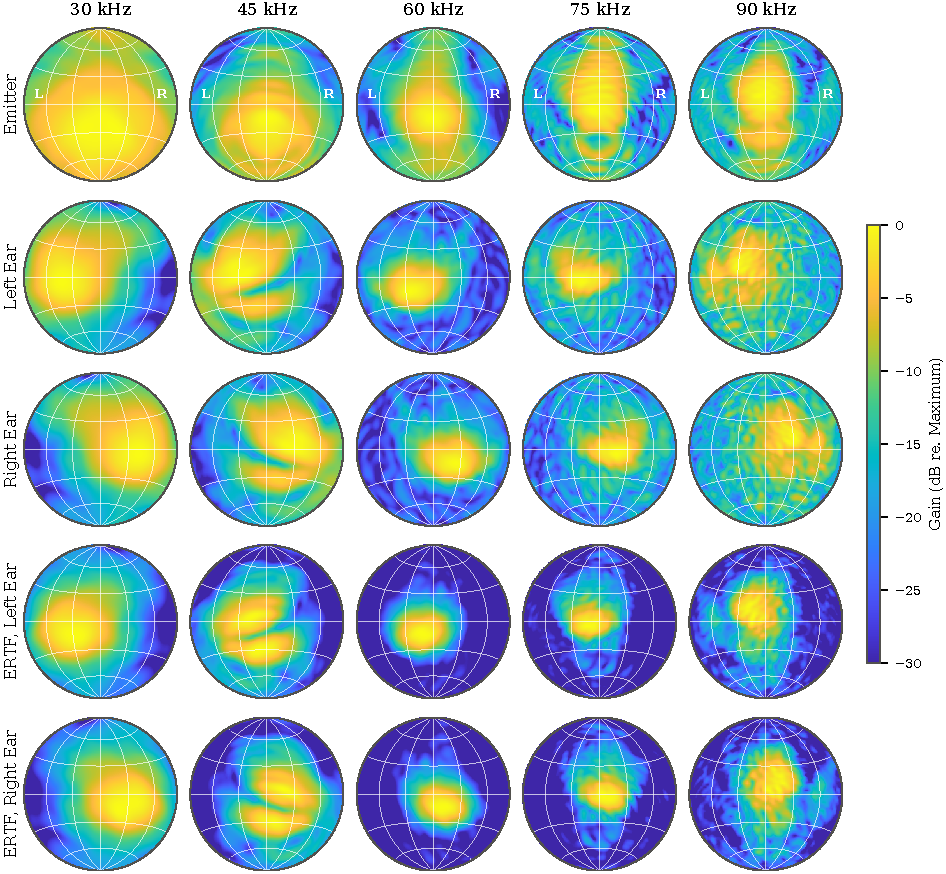
\includegraphics[width=0.86\linewidth]{figures/hrtfLaeap.pdf}
\caption{Directivity of the simulated sonar (Lambert azimuthal equal-area projection of the frontal hemisphere, seen from behind the head; grid lines every \SI{30}{\degree}). Rows: emitter, left ear, right ear and the ERTFs of both ears, at five frequencies between \SI{30}{\kilo\hertz} and \SI{90}{\kilo\hertz}, each normalized to its maximum.}
\label{fig:hrtf}
\end{figure*}

\subsection{Worlds and drives}
We used three simulated worlds (figure \ref{fig:worlds}). The main world is an \emph{indoor floor} of \SI{38}{\meter} by \SI{18}{\meter}, consisting of a grid of rooms separated by corridors of \SI{1.4}{\meter} to \SI{1.8}{\meter} wide, and a hall with 40 pillars. The walls carry 170 small reflectors (e.g., pipes and radiators), and to make aliasing explicit, we placed an identical pattern of three objects on two different corridor walls. The second world is a \emph{city} of \SI{46}{\meter} by \SI{26}{\meter} with the same topology but with streets of \SI{3}{\meter} to \SI{4}{\meter}, and the third is a small \emph{hall} used during development.

In the indoor floor and the city, the robot drives a random tour of about \SI{1}{\kilo\meter}, in which every corridor is driven at least twice in both directions, with a small lateral along the corridor wobble so that revisits are never exactly identical in position. A pulse is emitted every \SI{0.15}{\meter} of travel, yielding about 6400 pulses per drive. We developed and tuned the system on one route of the indoor floor, and used other random routes as unseen test cases. 

\begin{figure*}[t]
\centering
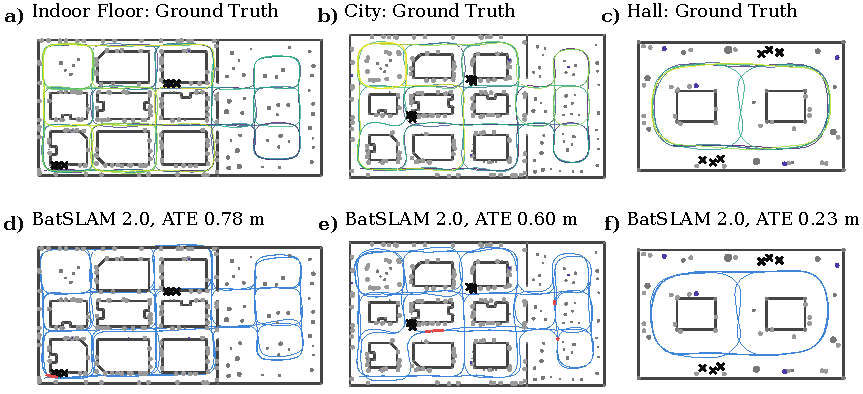
\includegraphics[width=\linewidth]{figures/worldsSlam.pdf}
\caption{The simulated worlds and exemplary results of BatSLAM 2.0. Top row: the ground-truth drive (colored from start to end) in a) the indoor floor (\SI{38}{\meter} by \SI{18}{\meter}, development drive on route 3, \SI{964}{\meter}), b) the city (\SI{46}{\meter} by \SI{26}{\meter}) and c) the small development hall (\SI{16}{\meter} by \SI{10}{\meter}). Black crosses: the two copies of the aliasing pattern. Bottom row, d)--f): the final map estimated by BatSLAM 2.0 for the same drives with calibrated odometry (blue), with its trajectory error (ATE); wrong links in the final graph are drawn in red.}
\label{fig:worlds}
\end{figure*}

\subsection{Odometry model}
The odometry was generated from the ground-truth increments with random noise (\SI{3}{\percent} forward, \SI{1}{\percent} lateral and \SI{1}{\degree} per $\sqrt{\si{\meter}}$ in heading) and a systematic error (a heading bias of \SI{0.6}{\degree\per\meter} and a scale error of \SI{2}{\percent}). We scaled the systematic part with a bias factor $b$: $b = 1$ represents uncalibrated wheel odometry, $b = 0.25$ a roughly calibrated robot and $b = 0$ a calibrated robot. Over \SI{1}{\kilo\meter}, dead reckoning drifts by \OdoDriftRange{}, depending on $b$ and the random seed. Typical robots in indoor environments can be assumed to have decently calibrated odometry, whereas in outdoor environments these calibrations are less accurate due to a higher prevalence of wheel slippage.

\subsection{Metrics}
As BatSLAM 2.0 builds a topological map, our primary criterion is the absence of wrong loop closures and map collapse rather than metric accuracy. The \emph{link precision} is the fraction of links for which query and anchor are truly within \SI{0.6}{\meter} and \SI{26}{\degree} of each other. The number of \emph{wrong commits} counts committed hypotheses of which the majority of links are wrong. The \emph{revisit coverage} is the fraction of true same-direction revisits that received a correct link. The \emph{collapsed pairs} are the fraction of node pairs that are at least \SI{4}{\meter} apart in reality, but less than half that distance apart in the map. Finally, we report the \emph{absolute trajectory error} (ATE) without alignment and after a rigid alignment in the plane.

The pose-graph part of BatSLAM 2.0 is implemented in Python using GTSAM 4.2 with Python bindings, and the simulator is implemented using custom MATLAB code. All experiments ran on a desktop computer with an AMD Ryzen 9 7900X.
